\documentclass[UTF8]{ctexbeamer}

\usetheme{Boadilla}
\usefonttheme[onlymath]{serif}

\usepackage{subfig}

% Title
\title{第3章 模型拟合}
\author{韩建伟}
\institute{
  信息学院\\
  \texttt{hanjianwei@zjgsu.edu.cn}
}
\date{2018/10/19}

\begin{document}

% Title page
\begin{frame}[plain]
  \titlepage{}
\end{frame}

\begin{frame}{分析数据集合的三个任务}
  刹车问题: $d_b=C_1v^2$, $d_b=C_2v$, 如何选择?

  \begin{description}
  \item[任务1] 按照一个或一些选出的模型类型对数据进行拟合.
    \begin{itemize}
    \item 必须明确最佳模型的含义,以及由此产生的需解决的数学问题.
    \end{itemize}
  \item[任务2] 从一些已经拟合的类型中选取最合适的模型.
    \begin{itemize}
    \item 为了比较不同类型的模型需要有一个判定准则.
    \end{itemize}
  \item[任务3] 根据收集的数据做出预报: 内插(第4章).
    \begin{itemize}
    \item 为了决定如何在观测的数据点间做出预测,也要明确一个判定准则.
    \end{itemize}
  \end{description}

\end{frame}

\begin{frame}{模型的拟合和内插之间的关系}
  \begin{description}
  \item[拟合] 接受模型和数据之间的某些偏差,以便有一个满意地解释所研究问题的模型. 强调为数据提供模型.
  \item[内插] 受数据的强力引导,曲线应该追踪数据的趋向,在数据点间做出预测. 对收集的数据给予了更大的信任,而较少注意模型的形式意义.
  \end{description}

  \begin{figure}
    \centering
    \subfloat[数据]{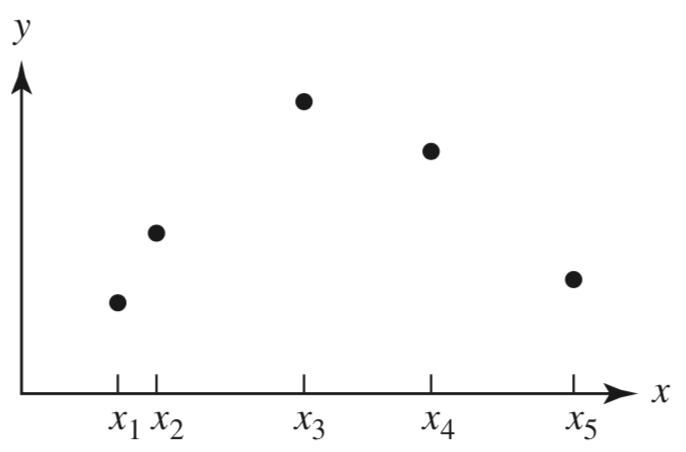
\includegraphics[height=.3\textheight{}]{data.png}}
    \subfloat[插值]{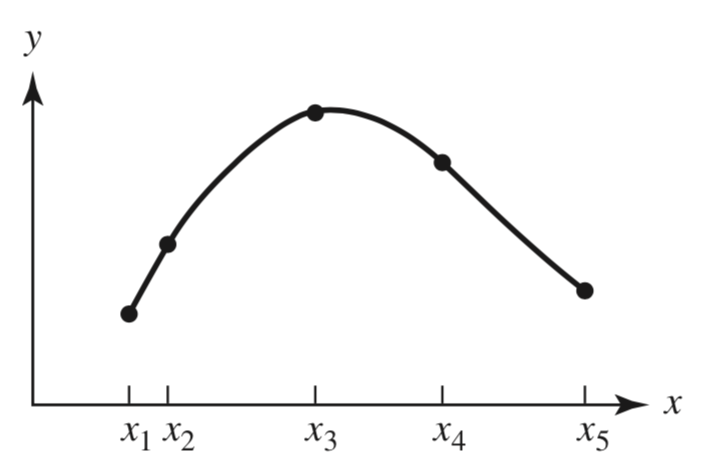
\includegraphics[height=.3\textheight{}]{interpolate.png}}
    \subfloat[拟合]{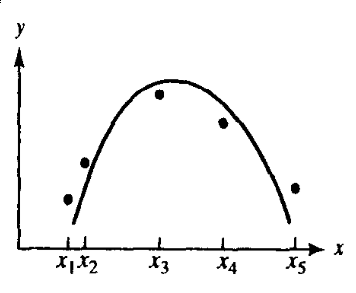
\includegraphics[height=.3\textheight{}]{fit.png}}
  \end{figure}
\end{frame}

\begin{frame}{建模过程中的误差来源}

  \begin{description}
  \item[公式化的误差] 可源于一些变量可忽略的假设条件,或在各种子模型中描述变量之间关系的过分简化.
  \item[截断误差] 归因于一个数学问题所用的数值方法.
  \item[舍入误差] 计算时使用有限小数位的机器引起的.
  \item[测量误差] 由数据收集过程中的不精确性引起的.
  \end{description}

\end{frame}

\begin{frame}{用图形为数据拟合模型}

  如何确定模型的参数? 收集数据!

  \begin{itemize}
  \item 采集多少个数据点?观察它们的费用和模型所要求的精度间进行平衡.
  \item 数据点的跨度. 自适应的数据采集密度.
  \item 将数据点看做是一个置信区间而不是一个单独的点.
  \end{itemize}
  
  \begin{figure}
    \centering
    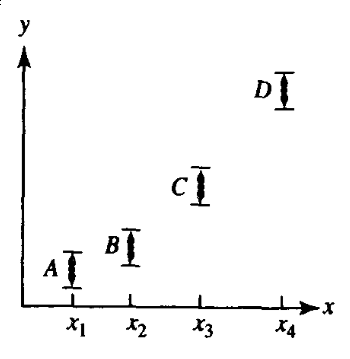
\includegraphics[height=.4\textheight{}]{confid.png}
  \end{figure}
  
\end{frame}

\begin{frame}{对原始数据拟合视觉观测的模型}
  \begin{figure}
    \centering
    \setcounter{subfigure}{0}{}
    \subfloat[极小化绝对偏差和]{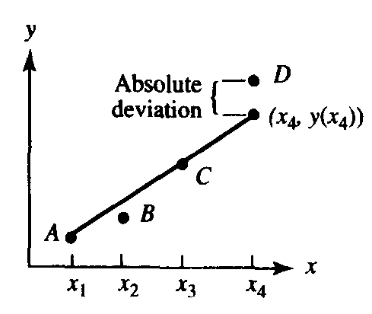
\includegraphics[height=.4\textheight{}]{abs.png}}
    \subfloat[极小化最大绝对偏差]{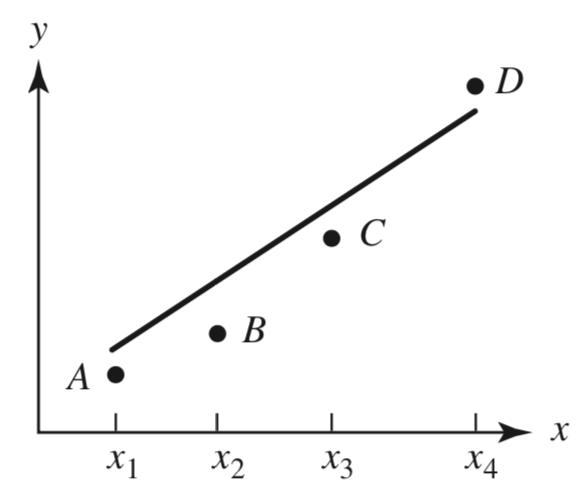
\includegraphics[height=.4\textheight{}]{large-abs.png}}
  \end{figure}

  视觉方法虽然不精确,但往往与建模过程的精度相称. 不要过分信任数值计算,视觉也是很重要的方法!

\end{frame}

\begin{frame}{变换数据}

  \begin{table}
    \centering
    \begin{tabular}{c|cccc}
      x & 1 & 2 & 3 & 4\\
      \hline{}
      y & 8.1 & 22.1 & 60.1 & 165
    \end{tabular}
    \caption{收集的数据}
  \end{table}

  \begin{figure}
    \centering
    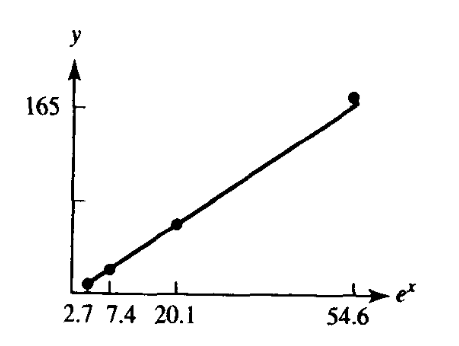
\includegraphics[height=.4\textheight{}]{y-exp.png}
    \caption{$y \propto e^x$}
  \end{figure}
\end{frame}

\begin{frame}{变换后的数据}

  \begin{table}
    \begin{tabular}{c|cccc}
      x & 1 & 2 & 3 & 4\\
      \hline{}
      $\ln{}$y & 2.1 & 3.1 & 4.1 & 5.1
    \end{tabular}
    \caption{变换后的数据: $y = Ce^x \Rightarrow \ln y = \ln C + x$}
  \end{table}

  \begin{figure}
    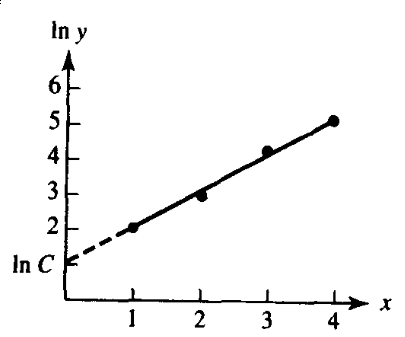
\includegraphics[height=.4\textheight{}]{lny.png}
    \caption{$\ln{}y \propto x$}
  \end{figure}
\end{frame}

\begin{frame}{数据变换}

  \begin{itemize}
  \item 变换过程中,距离发生了变换
  \item 选择一个好的变换非常重要
  \item $y = Ce^\frac{1}{x} \Rightarrow \ln y = \frac{1}{x} + \ln C$
  \end{itemize}

  \begin{figure}
    \centering
    \setcounter{subfigure}{0}{}
    \subfloat[收集的数据]{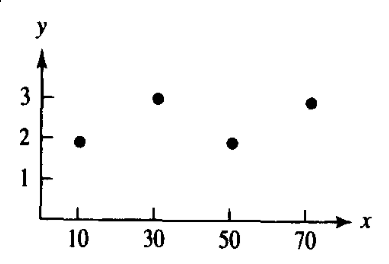
\includegraphics[height=.25\textheight{}]{collect-data.png}}
    \subfloat[变换后的数据点]{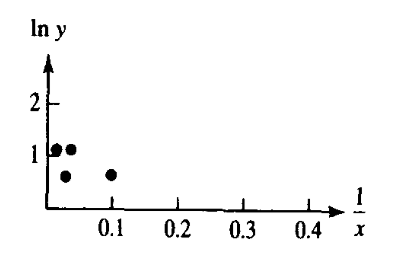
\includegraphics[height=.25\textheight{}]{trans-data.png}}
    \subfloat[拟合结果]{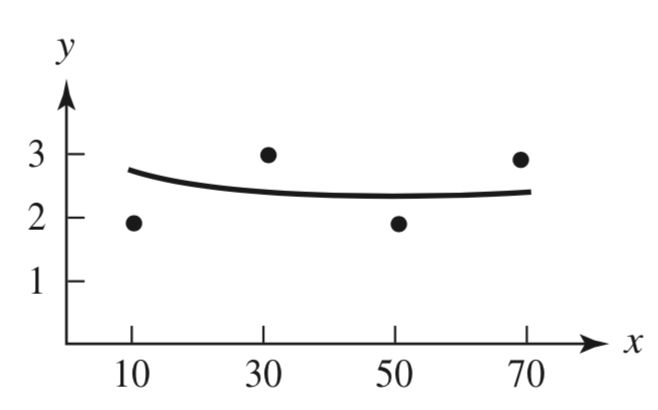
\includegraphics[height=.25\textheight{}]{fit-data.png}}
  \end{figure}
  
\end{frame}

\begin{frame}{模型拟合的解析方法}
  \begin{itemize}
  \item 切比雪夫近似准则
  \item 极小化绝对偏差之和
  \item 最小二乘准则
  \end{itemize}
\end{frame}

\begin{frame}{切比雪夫近似准则}
  \begin{block}{定义}
    给定某种函数类型$y=f(x)$和$m$个数据点$(x_i, y_i)$的一个集合,对整个集合极小化最大绝对偏差$|y_i - f(x_i)|$,即确定函数类型$y=f(x)$的参数从而极小化:
    \[
    Maximum |y_i - f(x_i)|,  i = 1, 2, .., m
    \]
  \end{block}

  \begin{itemize}
  \item 实际应用中通常很复杂.
  \item 应用这一准则所产生的最优化问题可能需要高级的数学方法,或者要用计算机数值方法.
  \end{itemize}

\end{frame}

\begin{frame}{极小化绝对偏差之和}
    \begin{block}{定义}
    给定某种函数类型$y=f(x)$和$m$个数据点$(x_i, y_i)$的一个集合,极小化绝对偏差$|y_i - f(x_i)|$之和,即确定函数类型$y=f(x)$的参数从而极小化:
    \[
    \sum_{i=1}^m |y_i - f(x_i)|
    \]
  \end{block}

  \begin{itemize}
  \item 由于出现了绝对值,这个和式的微分是不连续的.
  \end{itemize}

\end{frame}

\begin{frame}{最小二乘准则}
    \begin{block}{定义}
    给定某种函数类型$y=f(x)$和$m$个数据点$(x_i, y_i)$的一个集合,极小化绝对偏差$|y_i - f(x_i)|$之平方和,即确定函数类型$y=f(x)$的参数从而极小化:
    \[
    \sum_{i=1}^m |y_i - f(x_i)|^2
    \]
  \end{block}

  \begin{itemize}
  \item 运算简单,应用很广
  \end{itemize}
  
\end{frame}

\begin{frame}{谈谈准则}
  \begin{description}
  \item[极小化绝对偏差之和] 赋予每个数据点相等的权值来平均这些偏差
  \item[切比雪夫准则] 对潜在有大偏差的单个点给于更大的权值
  \item[最小二乘准则] 根据与中间某处的远近来加权,与单个点的偏离有关
  \end{description}

  \begin{itemize}
  \item 切比雪夫近似准则产生的偏差记为$c_i = |y_i - f_1(x_i)|, i=1,2,...,m$
  \item 最小二乘准则产生的偏差记为$d_i = |y_i - f_2(x_i)|, i=1,2,...,m$
  \item $d_{max} \ge c_{max}$
  \item $d_1^2+d_2^2+...+d_m^2 \le c_1^2+c_2^2+...+c_m^2 \le mc_{max}^2$
  \item $D=\frac{\sqrt{d_1^2+d_2^2+...+d_m^2}}{m} \le c_{max} \le d_{max}$
  \end{itemize}

\end{frame}

\begin{frame}{应用最小二乘准则拟合直线}
  \begin{block}{问题}
    设预期模型的形式为$y=Ax+B$, 并决定用$m$个数据点$(x_i, y_i)(i=1,2,...,m)$来估计$A$和$B$.
  \end{block}
  
  \begin{itemize}
  \item 用$y=ax+b$记作$y=Ax+B$的最小二乘估计,则要求极小化:
    \[
    S=\sum_{i=1}^m[y_i-f(x_i)]^2=\sum_{i=1}^m[y_i-ax_i-b]^2
    \]
  \item 最优的必要条件是:
    \[
    \frac{\partial S}{\partial a} = 0
    \]
    \[
    \frac{\partial S}{\partial b} = 0
    \]
  \end{itemize}
\end{frame}

\begin{frame}{应用最小二乘准则拟合直线}
  \[
  \frac{\partial S}{\partial a} = -2\sum_{i=1}^m(y_i-ax_i-b)x_i = 0
  \]
  \[
  \frac{\partial S}{\partial b} = -2\sum_{i=1}^m(y_i-ax_i-b) = 0
  \]
  重写这些方程:
  \[
  a\sum_{i=1}^mx_i^2 + b\sum_{i=1}^mx_i = \sum_{i=1}^mx_iy_i
  \]
  \[
  a\sum_{i=1}^mx_i + mb = \sum_{i=1}^my_i
  \]
\end{frame}

\begin{frame}{应用最小二乘准则拟合直线}
  \[
  a = \frac{m\sum x_iy_i - \sum x_i\sum y_i}{m\sum x_i^2 -(\sum x_i)^2} \Rightarrow \text{斜率}
  \]
  \[
  b = \frac{\sum x_i^2\sum y_i - \sum x_iy_i\sum x_i}{m\sum x_i^2 -(\sum x_i)^2} \Rightarrow \text{截距}
  \]

  \begin{itemize}
  \item 拟合幂曲线
  \item 经变换的最小二乘拟合
  \item 方法与直线拟合类似
  \end{itemize}
  
\end{frame}

\begin{frame}{选择一个好模型}

  \begin{table}
    \centering{}
    \begin{tabular}{c|ccccc}
      x & 0.5 & 1.0 & 1.5 & 2.0 & 2.5\\
      \hline{}
      y & 0.7 & 3.4 & 7.2 & 12.4 & 20.1
    \end{tabular}
    \caption{数据}
  \end{table}

  \begin{table}
    \centering{}
    \begin{tabular}{cccc}
      准则 & 模型 & $\sum{}[y_i - y(x_i)]^2$ & $Max |y_i - y(x_i) |$\\
      \hline{}
      最小二乘 & $y=3.1869x^2$ & 0.2095 & 0.3476\\
      变换后最小二乘 & $y=3.1368x^2$ & 0.3633 & 0.4950\\
      切比雪夫 & $y=3.17073x^2$ & 0.2256 & 0.28293
    \end{tabular}
    \caption{模型对比}
  \end{table}

\end{frame}

\begin{frame}{如何评价模型}
  \begin{itemize}
  \item 根据偏差进行选择
  \item 以具体个案为基础,要考虑模型的目的、实际情况要求的精度、数据的准确性以及使用模型时独立变量值的范围
  \item 视觉方法(从图中观察)
  \item 数据收集的不够就无法为进一步的模型求精提供保证
  \end{itemize}

  试用本章方法分析上一节课的刹车问题.

\end{frame}

\end{document}

%%% Local Variables: 
%%% TeX-master: t
%%% TeX-engine: xetex
%%% End: 
